\section{Theorie}
\label{sec:Theorie}
Eine Spannungsquelle liefert über einen endlichen Zeitraum eine konstante elektrische Leistung.
Die Leerlaufspannung $U_0$ liegt genau dann an den Klemmen der spannungsquelle an, wenn kein Strom fließt.
Falls über einen äußeren Lastwiderstand $R_a$ Strom fließt, so sinkt die Leerlaufspannung auf
die Klemmspannung $U_k$ ab.

\begin{figure}[H]
  \centering
  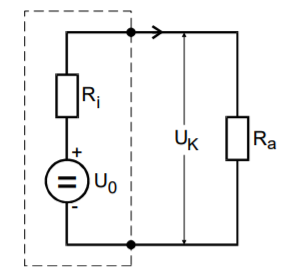
\includegraphics[height=5cm]{bild1.PNG}
  \caption{Darstellung einer Spannungsquelle mit Lastwiderstand}
  \label{fig:RLC-Kreis(mit Widerstand)}
\end{figure}


Dies ist mit dem zweiten kirchhoff'schen Gesetz erklärbar:
\begin{equation}
  \sum_{n} U_{0_n} = \sum_{m} R_m I_m
\end{equation}

Mit $U_0 = IR_j + IR_a$ folgt für die Klemmspannung:
\begin{equation}
  U_k = IR_a = U_0 - IR_j
\end{equation}

$R_j$ ist dabei der Innenwiderstand der Spannungsquelle.
Für hochohmige Voltmeter geht $IR_a$ gegen $0$ und somit $U_k$ gegen $U_0$, weshalb zur Messung der Leerlaufspannung
diese verwendet werden sollten.

Der Innenwiderstand von elektrischen Generatoren ist nicht unbedingt durch einen Gleichstromwiderstand gegeben, weshalb
der innenwiderstand dann differentiell ausgedrückt wird:
\begin{equation}
  R_j = \frac{\symup{d}U_k}{\symup{d}I}
\end{equation}

Die Spannungsquelle kann wegen des Innenwiderstandes keine beliebig hohe elektrische Leistungen
abgeben. Die elektrische Leitung ist gegeben durch:
\begin{equation}
  N = I^2 R_a = N(R_a)
\end{equation}

Für $R_a = R_j$ wird die Leistung maximal, wobei dann von Leistungsanpassung gesprochen wird.
